\documentclass{beamer}
\usepackage[utf8]{inputenc}
\usepackage{epstopdf}
\usetheme[pageofpages=/,% String used between the current page and the
                         % total page count.
          bullet=circle,% Use circles instead of squares for bullets.
          titleline=true,% Show a line below the frame title.
          alternativetitlepage=true,% Use the fancy title page.
          titlepagelogo=logo_afonso,% Logo for the first page.
          watermark=Minerva_UFRJ_Black_transparency,% Watermark used in every page.
          watermarkheight=90px,% Height of the watermark.
          watermarkheightmult=4,% The watermark image is 4 times bigger
                                % than watermarkheight.
          ]{Torino}
\usepackage[brazil]{babel}

\author{\textbf{Alunos: \newline
		Cayo Valsamis \newline
		Gabriel Pelielo \newline
		Rafael Accácio \newline
		Rodrigo Moysés}}
\title{\textbf{Introdução à Otimização \vspace{0.25cm} \newline 
		       Trabalho 2}}
\institute{Universidade Federal do Rio de Janeiro}
\date{19 de Janeiro, 2016}

\begin{document}
	
	\setbeamertemplate{section in toc}[square]
	
	\AtBeginSection[]{
		\begin{frame}
			\frametitle{Sumário}
			\tableofcontents[currentsection]
		\end{frame}
	}
	
	
	\begin{frame}[t,plain]
		\titlepage
	\end{frame}
	
	\begin{frame}{Sumário}
		\tableofcontents
	\end{frame}
	
	%O trabalho detalhado neste relatório se baseia em analisar métodos numéricos para realizar busca de mínimos de funções vetoriais. Foram implementados cinco métodos diferentes de localização de mínimos:

\begin{itemize}
	\item Método da Descida Máxima (ou gradiente)
	\item Método do Gradiente Conjugado
	\item Método de Newton
	\item Método de Newton Modificado
	\item Método de Quase Newton
\end{itemize}

Todos os métodos foram implementados na plataforma \textit{MATLAB}, através de um programa de interface gráfica usado para escolher o método desejado e inserir alguns valores necessários para executar a busca. O objetivo do trabalho foi comparar esses métodos de acordo com os quesitos de tempo de execução, número necessário de iterações e por fim qualificá-los de acordo com cada função inserida.
	%\tableofcontents
	
	
	\section{Descida Máxima}
	O método de Descida máxima, ou método do gradiente, se baseia em um método muito simples para encontrar o mínimo de uma função.
 A partir de um ponto inicial calcula-se a direção de maior de crescimento, de descida máxima ou sentido inverso do gradiente, que dão nome ao método, 
e faz-se um avanço nessa mesma direção.\\
 
Como sabemos, o gradiente de uma função representa sua direção de maior crescimento. Sabendo disso utiliza-se a direção oposta, 
mas a questão que fica é qual o avanço é necessário. Para resolver isso, a direção do gradiente foi normalizada, $d^k$, e criou-se uma variável, $\alpha$, que indica o avanço a ser feito. 

Com o gradiente calculado naquele ponto, usa-se um método de minimização unidimensional qualquer para minimizar a função $x^k - \alpha d^k$. 
Foi escolhido o método da seção áurea, devido a sua grande flexibilidade e por encontrar o mínimo com poucas iterações e baixo esforço computacional. 
Após a minimização utilizamos o valor de $\alpha$ que a minimiza como avanço.
\\
Dessa forma faz-se a iteração para encontrar o próximo ponto, que a princípio 
está mais perto do mínimo. E assim faz-se até convergir ao ponto de mínimo da função (considerando que a mesma o possui).

Como métodos de parada foram escolhidos o tamanho da norma do vetor diferença de gradiente em cada iteração, a norma entre a diferença entre os pontos em cada iteração e finalmente o número de iterações.

Para verificar a convergência do método vemos como são as direções de avanço do algoritmo e também sua norma. Sabe-se a partir de \cite{Notastioafel} que cada iteração tem direção perpendicular a anterior e que a convergência dá-se quando cada avanço é menor que o anterior, assim como vemos na figura \ref{fig:stegradeszigzag}


\begin{figure}[H]
	\begin{center}
		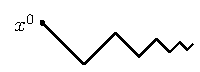
\includegraphics[width=8cm]{../tikz/stegrades}  
		\caption{Representação do avanço convergente em zig-zag com ângulos retos.}
		\label{fig:stegradeszigzag}
	\end{center}
\end{figure}


	\begin{quote}
		\centering
		Lei de Iteração:
	\end{quote}

\begin{equation}
	x^{k+1} = x^k - \alpha d^k
	\end{equation}
	
Após construir o algoritmo, foram feitos testes usando algumas funções:

\begin{itemize}
	\item $ f_1(x,y) = x^2 + y^2$
	\item $ f_2(x,y) = -e^{-x^2 -y^2}$
	\item $ f_3(x,y) = cos(\frac{xy}{5})+sin(\frac{xy}{5}) $
	\item $ f_4(x,y) = |x+y| $
\end{itemize}


\newpage

\begin{figure}[H]
	\begin{center}	
		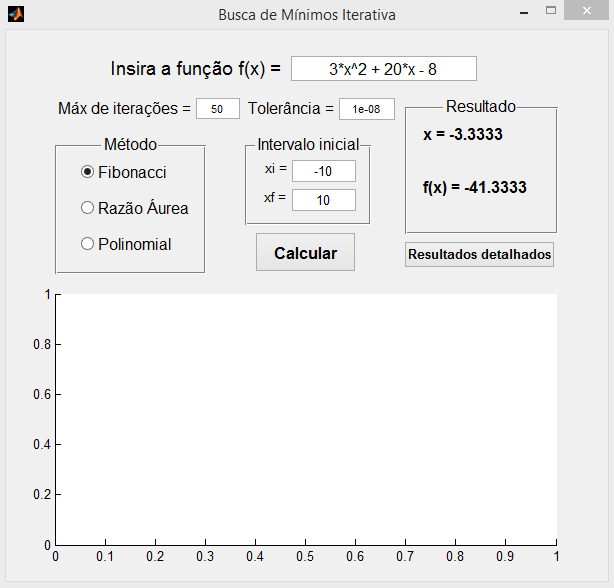
\includegraphics[width=12cm]{../stegrades/f1_gui.PNG}
		\caption{Janela de inicialização de $ f_1(x,y) $}
		\label{fig:f1_gui}
	\end{center}
\end{figure}



\begin{figure}[H]
	\begin{center}	
		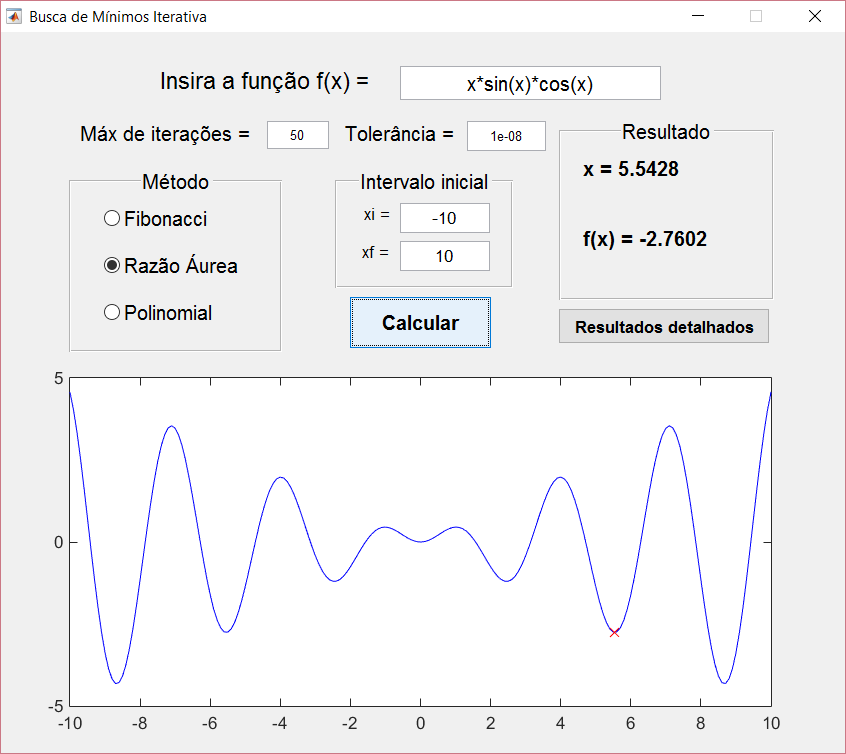
\includegraphics[width=12cm]{../stegrades/f2_gui.PNG}
		\caption{Janela de inicialização de $ f_2(x,y) $}
		\label{fig:f2_gui}
	\end{center}
\end{figure}



\begin{figure}[H]
	\begin{center}	
		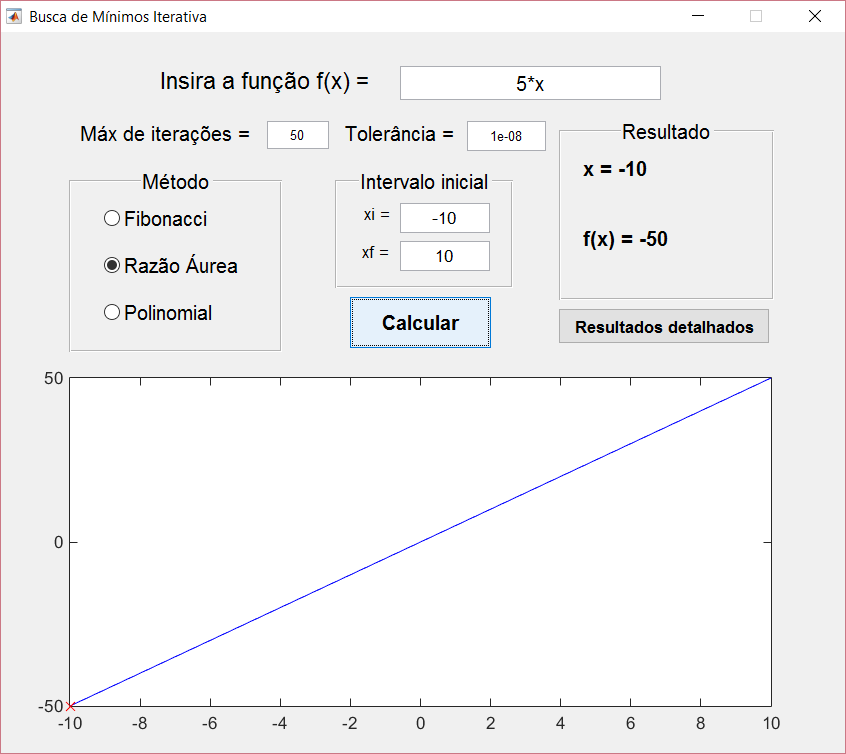
\includegraphics[width=12cm]{../stegrades/f3_gui.PNG}
		\caption{Janela de inicialização de $ f_3(x,y) $}
		\label{fig:f3_gui}
	\end{center}
\end{figure}



\begin{figure}[H]
	\begin{center}	
		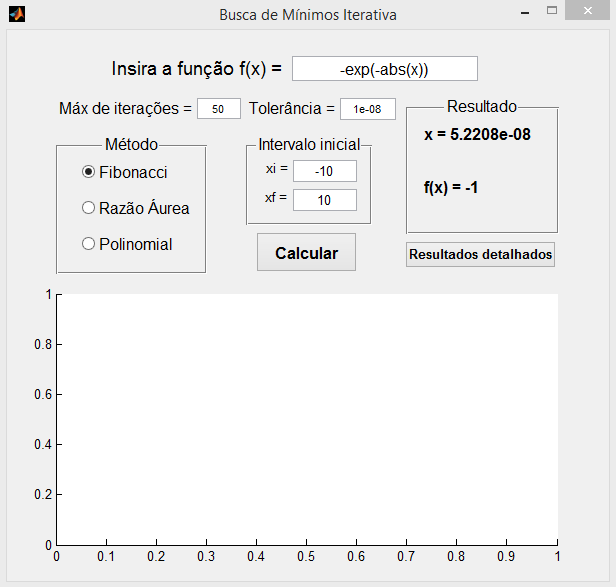
\includegraphics[width=12cm]{../stegrades/f4_gui.PNG}
		\caption{Janela de inicialização de $ f_4(x,y) $}
		\label{fig:f4_gui}
	\end{center}
\end{figure}






\newpage




	
	
	\section{Gradiente Conjugado}
	\begin{frame}{Gradiente Conjugado}
	\vspace{-22mm}
	\begin{itemize}
		\item Suaviza as mudanças de direção abruptas do método do gradiente.
		\vspace{5mm}
		\item Adição do coeficiente de inércia $\beta$ conserva uma fração da direção anterior.
	\end{itemize}
	\vspace{5mm}
	\begin{equation}
	d^{k+1} = -g(x^{k+1}) + \beta_k d^k
	\end{equation}

\end{frame}

\begin{frame}{Gradiente Conjugado - coeficientes}
	O avanço $\alpha$ tem a seguinte fórmula:
		\begin{align}
			x^{k+1} &= x^k + \alpha_k d^k \\
			\tilde{f}(\alpha) &= f(x^k + \alpha d^k)
		\end{align}
		A função $\tilde{f}(\alpha)$ é minimizada utilizando a razão áurea.\\
		Já o coeficiente $\beta$ é uma relação entre o gradiente atual e o anterior.\\
		Segundo \textit{Polak-Rebière}:
		\begin{equation}
			\beta_k = \frac{||g^{k+1}|| - [g^+1]^T g^k}{||g^k||}
		\end{equation}

\end{frame}
	
	\section{Newton}
	\begin{frame}{Método de Newton}
	Os métodos de Newton se baseiam em encontrar uma aproximação quadrática $ q(x) $ a partir do teorema de Taylor para a função objetivo $ f(x) $, e assim, encontrar o seu mínimo.
	
	\begin{quote}
		\centering
		Lei de Iteração:
	\end{quote}

	\begin{equation}
	x^{k+1} = x^k - [G^k]^{-1}g^k
	\end{equation}
	
	
\end{frame}	
	
	\section{Newton Modificado}
	\begin{frame}{Newton Modificado}
	
	Para melhorar o método de Newton, foram feitas algumas alterações, como:
	
	\begin{itemize}
		\item Diminuição do avanço na direção $ d^k $, da forma:
	\end{itemize}
	
	\begin{equation}
	x^{k+1} = x^k + \alpha_k d^k
	\end{equation}
	
	onde $ \alpha_k $ minimiza $ \tilde{f}(\alpha) = f(x^k + \alpha d^k) $
	
\end{frame}


\begin{frame}{Newton Modificado}
	
	\begin{itemize}
		\item Correção do sinal da Hessiana por um truque matricial:
	\end{itemize}	
	
	\begin{equation}
	F^k = G^k + \gamma I_n
	\end{equation}
	
	Em que $ F^k $ tem autovalores positivos para poder gerar uma direção $ d^k $ de descida da forma
	
	\begin{equation}
	d^k = -[F^k]^{-1}g^k = -[\nabla^2 f(x^k) + \gamma I_n]^{-1}\nabla f(x^k)
	\end{equation}
	
\end{frame}
	
	\section{Quase Newton}
	\begin{frame}{Método de Quase Newton}
	Todos os métodos de Newton baseiam-se em facilitar o cálculo da Hessiana. O método de Quase Newton diferencia-se por apoiar-se na chamada "Condição de Quase Newton":
	\\
	\begin{equation}
		H^{k+1} \gamma^{k} = \delta^{k} = \left\{
		\begin{tabular}{c}
		\gamma^{k} = g^{k+1} - g^{k}\\
		\delta^{k} = x^{k+1} - x^{k} 
		\end{tabular}
	\end{equation}
\end{frame}

\begin{frame}	
Duas possibilidades para se gerar matrizes H satisfazendo essa restrição são o método de Davidon-Fletcher-Powell (DFP):
\begin{equation}
	H^{k+1} = H - \frac{H \gamma \gamma^T H}{\gamma^T H \gamma} + \frac{\delta \delta^T}{\delta^T \gamma}
\end{equation}	

ou o método de Broyden-Fletcher-Goldfarb-Shanno (BFGS)

\begin{equation}
H^{k+1} = H - \frac{\delta \gamma^T H + H \gamma \delta^T}{\delta^T \gamma} + \Bigg( 1 + \frac{\gamma^T H \gamma}{\delta^T \gamma}\Bigg) \frac{\delta \delta^T}{\delta^T \gamma}
\end{equation}	


\end{frame}
	
	\section{Programa}
	bla bla bla
	
	\section{Conclusão}
	bla bla bla
	
\end{document}